\chapter{Results}
In this section we present and compare results of the six models aplied in STLF. The performance of the models are evaluated using MAPE, MAE, RMSE and $R^2$. These metrics can give us a clear picture and comparisons framework for each of the model performance.  The goal is to represent the accuracy, robustness and suitability of the ML and AI models to solve STLF.




\section{Dataset Preprocessing Results}
 The continuous\_dataset.csv contained continuous time series data. The empty slots were filled using the forward and back-filling process.Figure \ref{fig:originaldataset}
 \begin{figure}[h]
 	\centering
 \begin{minipage}[b]{0.45\linewidth}
 	\centering
 	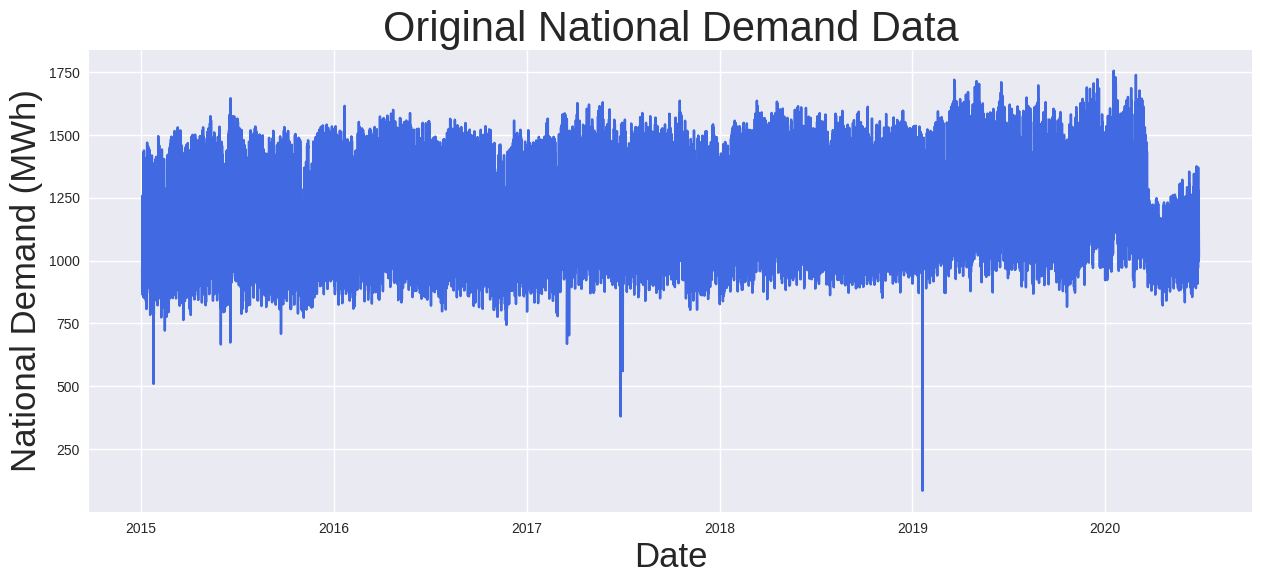
\includegraphics[width=\linewidth]{Chapters/images/results/original_dataset}
 	\caption{The original national demand .}
 	\label{fig:originaldataset}
 \end{minipage}
 \begin{minipage}[b]{0.45\linewidth}
 	\centering
 	\includegraphics[width=\linewidth]{"Chapters/images/results/train test split_after HI"}
 	\caption{HI processed dataset with traintest split.}
 	\label{fig:train-test-splitafter-hi}
 \end{minipage}
 \end{figure}
 
 The HI method explained in section \ref{sec:HI_method}, was used to handle outliers in the dataset, fixing all data-points that deviated from the normalcy.  After implementing the HI-method the train test split of 80/20 was implemented with a validation set ratio of 0.2 of the testing data. Figure \ref{fig:train-test-splitafter-hi} shows the effectiveness of the HI method in removing noisy details in the dataset.

 \begin{figure}[h]
  	\centering
  	% First figure
  	\begin{minipage}[b]{0.45\linewidth}
  		\centering
  		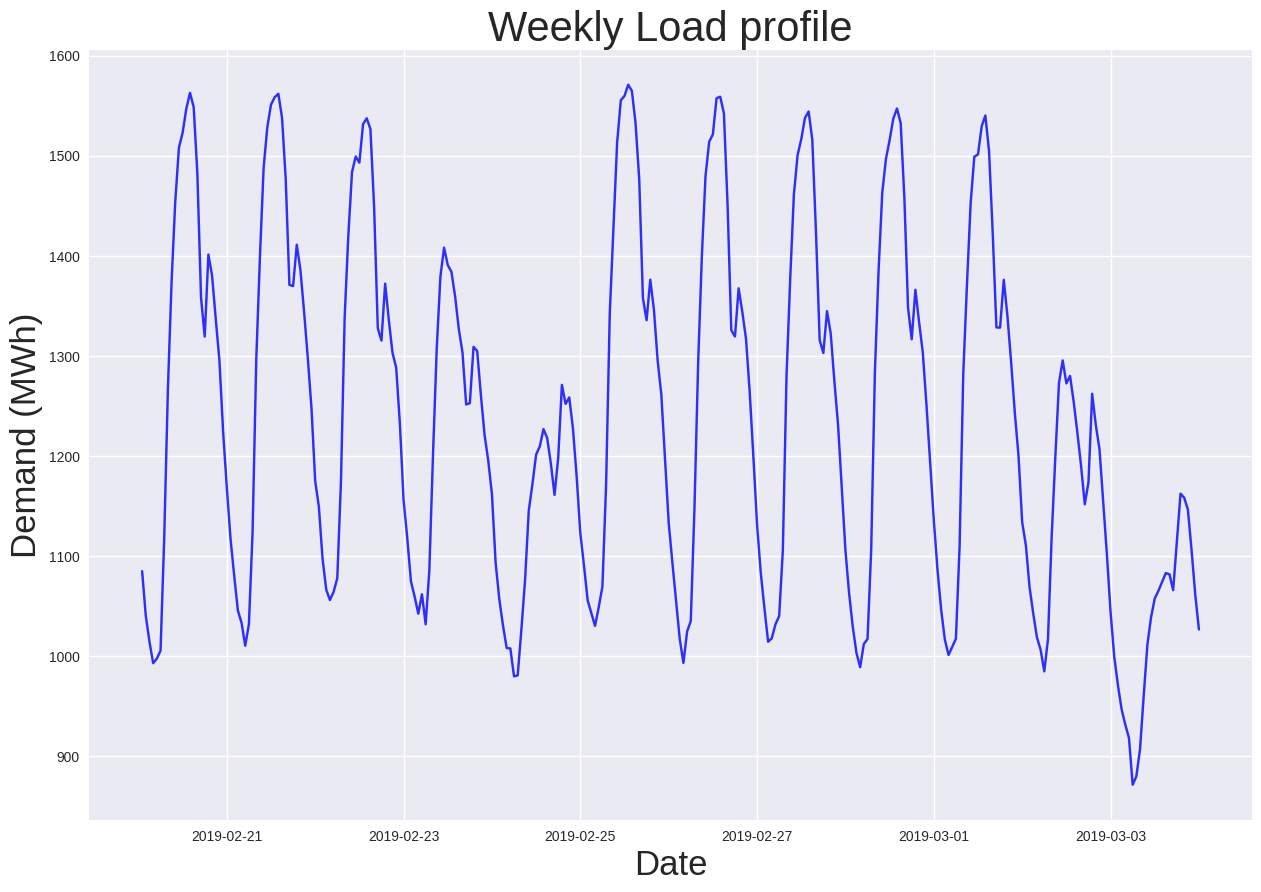
\includegraphics[width=\linewidth]{Chapters/images/results/weekly_load_profile.png}
  		\caption{The general weekly national load profile.}
  		\label{fig:weeklyloadprofile}
  	\end{minipage}
  	\hfill
  	% Second figure
  	\begin{minipage}[b]{0.45\linewidth}
  		\centering
  		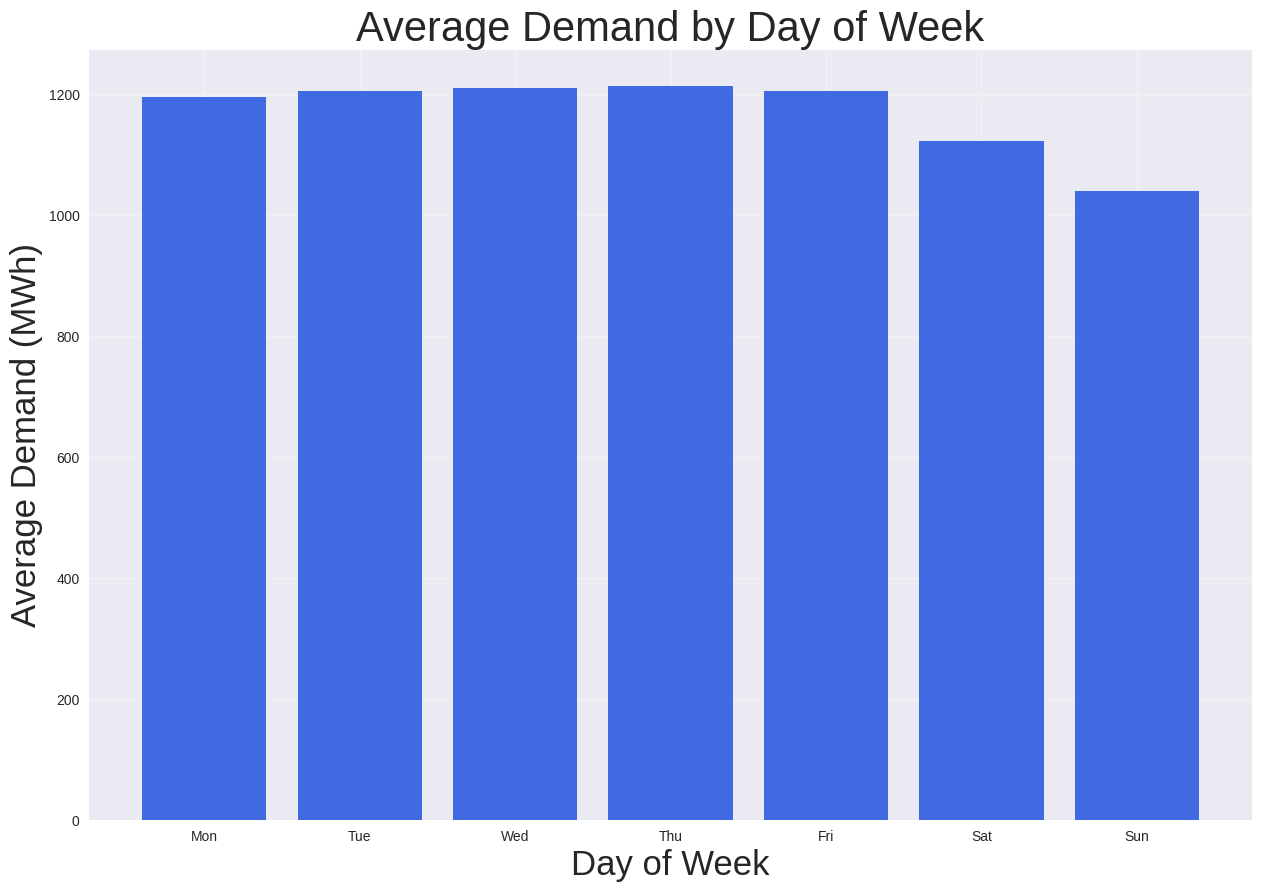
\includegraphics[width=\linewidth]{Chapters/images/results/average_daily_demand.png}
  		\caption{The weekly average daily demand }
  		\label{fig:averagedailydemand}
  	\end{minipage}
  \end{figure}
  
  
The weekly load profile in figure \ref{fig:weeklyloadprofile} shows a daily pattern that the load exhibits.The trend shows a higher usage during the week and lower usage in the weekend, with the lowest usage day being Sunday. This phenomenon represents a load profile that is found in places with industries that has maximum load requirements during the day. Figure \ref{fig:averagedailydemand} shows the average daily demand  of electricity. It also shows a higher usage during the week and lower consumption on the weekend, with Sunday being the lowest consumption day. 
  \begin{figure}[h]
  	\centering
  	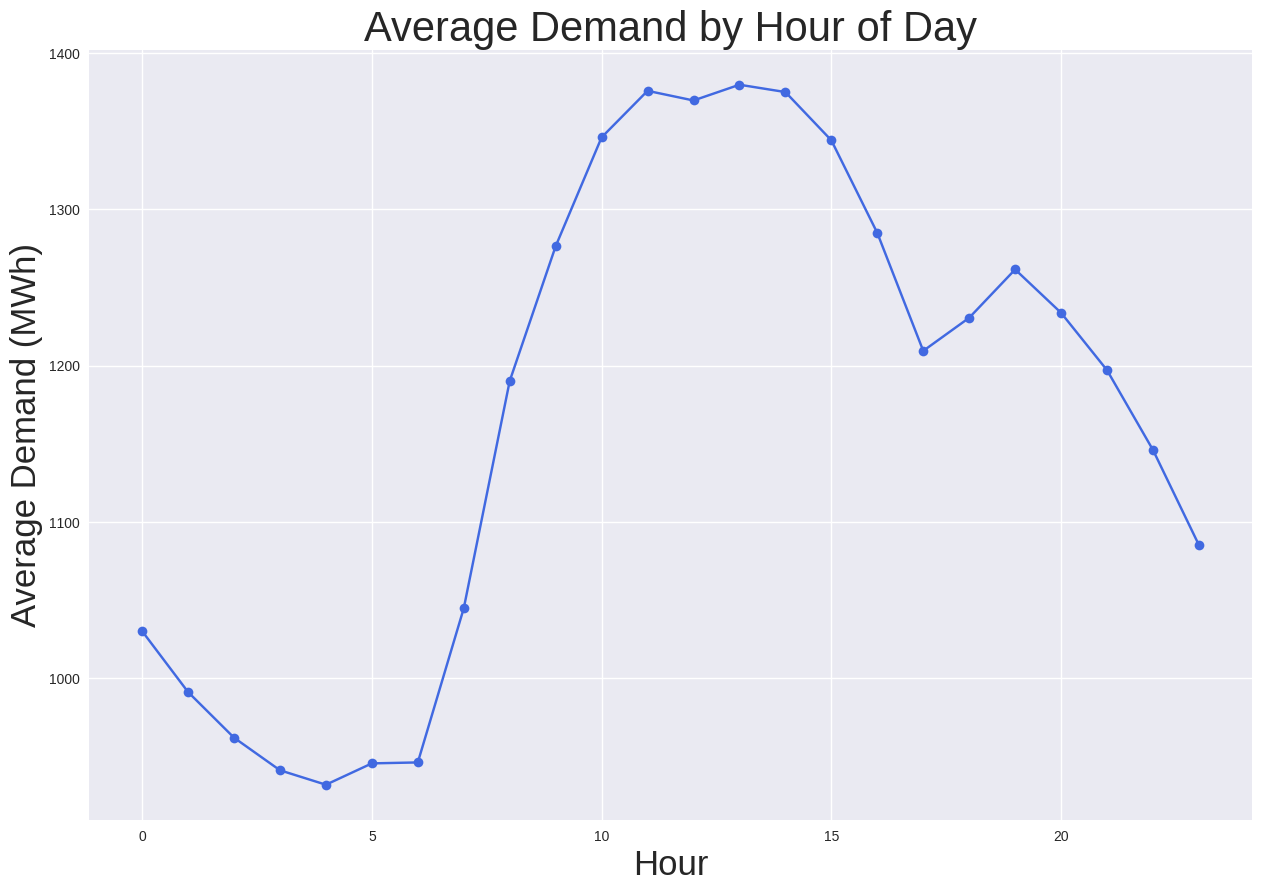
\includegraphics[width=0.45\linewidth]{Chapters/images/results/average_hourly_demand}
  	\caption{Average hourly demand of electricity between 2015 and 2020 in panama}
  	\label{fig:averagehourlydemand}
  \end{figure}
  
  Figure \ref{fig:averagehourlydemand} shows the average hourly usage of data. The averages show that the lowest consumption is in the early hours of the day, with a steady rise in the early morning leading to a peak at midday. After midday there is a steady decrease in demand with a slight increase between the 18th and 20th hour of the day, this is followed by a drop in usage leading to the early hours of the day.  


\section{Model Simulation Results}

\subsection{Statistical Model : Exponential smoothing}
\subsubsection{Model Choice result}
The algorithm in Appendix \ref{sec:appendixA}, figure \ref{fig:exponential-smoothing-model-choice} was used to find the best model to use for the ES model. Table \ref{tab:es_model_selection} shows the ES models and a parameters that were tested to find the best model.

\begin{table}[ht]
	\centering
	\resizebox{\textwidth}{!}{%
		\begin{tabular}{lccccccc}
			\hline \\
			\textbf{Model} & \textbf{Trend} & \textbf{Seasonality} & \textbf{Seasonality Period} & \textbf{Damped} & \textbf{MAPE (\%)} & \textbf{MSE (MWh)} & \textbf{AIC}
			\\
			\hline
			Simple               & None  & None & –  & No  & 13.76\%  & 180.98 & 343990.96 \\
			Double               & Add   & None & –  & No  & 15.14\%  & 172.11 & 327001.68 \\
			Triple\_Add          & Add   & Add  & 24 & No  & 10.56\%  & 125.56 & 277981.02 \\
			Triple\_Mul          & Mul   & Mul  & 24 & No   & 34.48\%  & 408.23 & 272265.85 \\
			Triple\_Add\_Damped  & Add   & Add  & 24 & Yes &  9.99\%  & 120.81 & 277708.98 \\
			Triple\_Mul\_Damped  & Mul   & Mul  & 24 & Yes & 10.01\%  & 119.49 & 272266.18 \\
			\hline
		\end{tabular}%
	}
	\caption{Exponential Smoothing Models chosen for benchmarking and their performance (Add = Additive , Mul = Multiplicative).}
	\label{tab:es_model_selection}
\end{table}

The best performing ES model was the Triple Multiplicative Damped algorithm, which uses a seasonality period of 24 to capture daily recurring patterns. While the MAPE and MSE values for Triple\_Add\_Damped and Triple\_Mul\_Damped are very close, the lower AIC of Triple\_Mul\_Damped indicates a better overall model fit. This model was selected as the benchmark for evaluating other forecasting approaches in this study.

\subsubsection{ES model Results}
The ES model achieved a MAPE of 9.57\% with a MAE of 118.14Mwh using the Triple Multiplicative Damped configuration. Table \ref{tab:exp_smoothing_results} summarizes the model performance metrics. 
\begin{table}[h!]
	\centering
	\caption{Triple Multiplicative Damped Exponential Smoothing Model Parameters and Results}
	\label{tab:exp_smoothing_results}
	\begin{tabular}{ll}
		\hline
		\textbf{Metric / Parameter} & \textbf{Value} \\
		\hline
		\multicolumn{2}{l}{\textbf{Model Results}} \\
		AIC & 20118 \\
		MAPE (Mwh) &  9.57\% \\
		MAE (Mwh) & 118.14 \\
		RMSE (Mwh) & 141.84 \\
		$R^2$ & 0.5241\\
		\hline
	\end{tabular}
\end{table}
These parameters produced the best results among the ES models tested, as determined by the selection algorithm shown in Figure \ref{fig:exponential-smoothing-model-choice} in Appendix \ref{sec:appendixA}.
\begin{figure}[h!]
	\begin{minipage}[b]{0.45\linewidth}
	\centering
	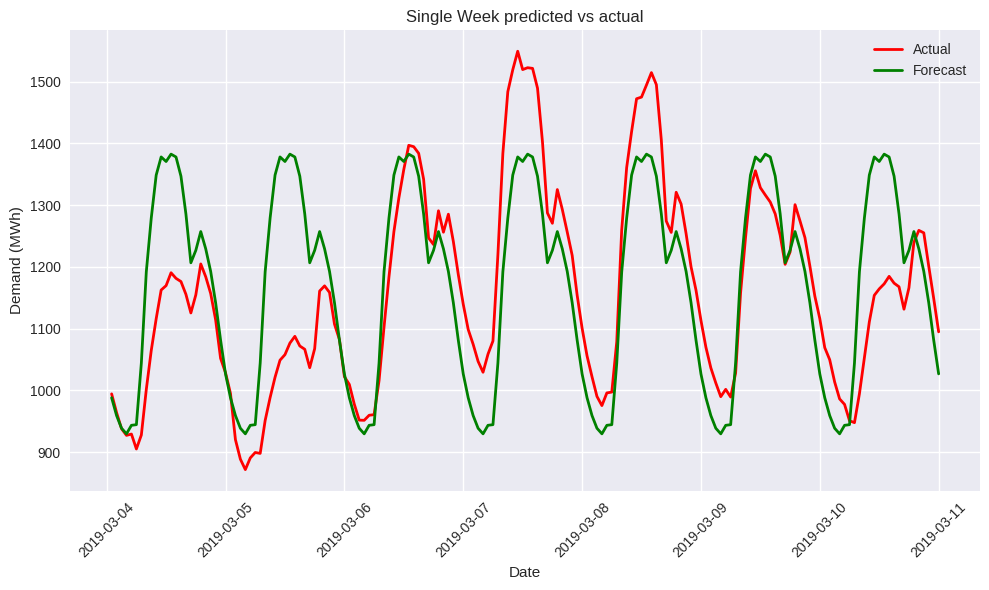
\includegraphics[width=\linewidth]{Chapters/images/results/ES_predicted_vs_actual}
	\caption{The ES predicted results against the actual demand in a week}
	\label{fig:espredictedvsactual}
\end{minipage}
\hfill
% Second figure
\begin{minipage}[b]{0.45\linewidth}
	\centering
	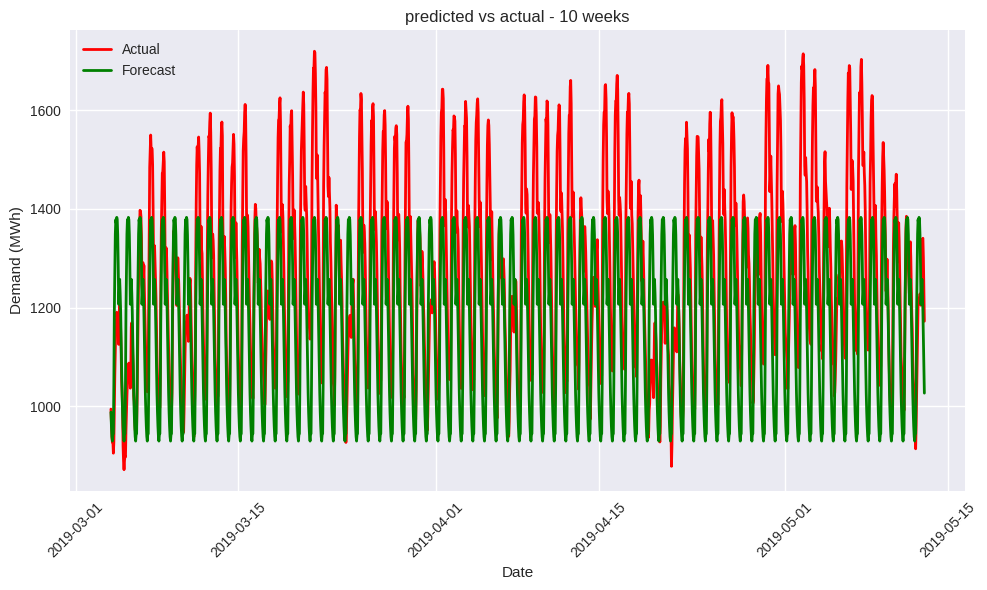
\includegraphics[width=\linewidth]{Chapters/images/results/ES_predicted_vs_actual_10weeks}
	\caption{ES model predicted vs actual load demand over 10 weeks}
	\label{fig:espredictedvsactual10weeks}
	
\end{minipage}
\end{figure}
 Figures \ref{fig:espredictedvsactual} and \ref{fig:espredictedvsactual10weeks} compare the predicted and actual load values. Figure \ref{fig:espredictedvsactual} illustrates the model’s ability to capture the training data patterns; however, it shows limited responsiveness to changing demand features. Figure \ref{fig:espredictedvsactual10weeks} highlights the model’s performance over a longer period, indicating limited generalization, which is consistent with the known limitation of ES models when handling nonlinear and complex time series data.
 
 \subsection{Machine Learning  : XGBoost Model Results}
 
The XGBoost model achieved a MAPE of 1.60\% and an $R^2$ value of 0.979, demonstrating excellent predictive performance and strong correlation with the actual load demand. The model’s gradient boosting framework iteratively minimizes residual errors at each boosting stage, leading to highly accurate forecasts particularly when the test data closely resembles the training distribution.


 \begin{table}[h!]
 	\centering
 	\small
 	\caption{Comparison of XGBoost Results with Different Data Processing Techniques}
 		
 	\resizebox{\textwidth}{!}{%
 	\begin{tabular}{lcccc}
 		\hline
 		\textbf{Metric} & \textbf{No Data Processing} & \textbf{Cyclical Encoding (CE)} & \textbf{Only Lag Features} & \textbf{Lag + CE} \\
 		\hline
 		MSE(Mwh)   & 20358  & 12861  & 1519   & 873   \\
 		RMSE(Mwh)  & 143.00 & 113.40 & 38.97  & 29.55 \\
 		MAE(Mwh)   & 115.27 & 91.57  & 27.15  & 18.58 \\
 		MAPE (\%) & 9.46   & 7.65   & 2.34   & 1.64  \\
 		\hline
 	\end{tabular}
 }
 	\label{tab:xgboost_comparison}
 \end{table}
 Table \ref{tab:xgboost_comparison} presents a comparison of XGBoost performance under different data preprocessing techniques. The inclusion of lag features and cyclical encoding significantly enhanced the model’s accuracy, reducing the MSE from 20,358 MWh (no preprocessing) to just 873 MWh when both preprocessing methods were applied. Similarly, the MAPE improved from 9.46\% to 1.64\%, highlighting the importance of feature engineering in improving model generalization.

Figure \ref{fig:xgboostoutput} illustrates the comparison between the predicted and actual load values. The model closely follows the true demand pattern, indicating its strong ability to capture nonlinear relationships and adapt to temporal variations in the load data.
 \begin{figure}[h!]
 	\centering
 	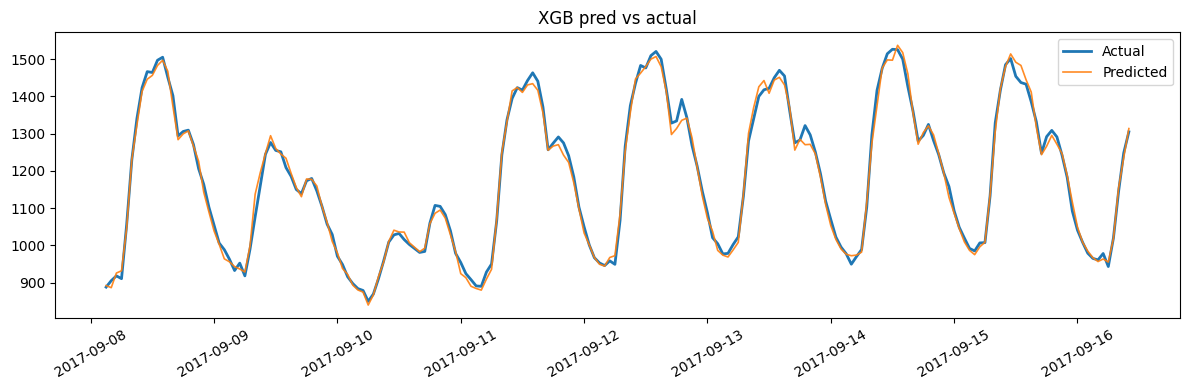
\includegraphics[width=0.75\linewidth]{Chapters/images/results/xgboost_output}
 	\caption{Comparison of XGBoost with the actual load}
 	\label{fig:xgboostoutput}
 \end{figure}
Overall, the XGBoost model demonstrated superior performance compared to traditional statistical models, largely due to its ensemble learning mechanism and the effectiveness of feature engineering applied during data preprocessing.


 
 \subsection{Deep Learning : DBN Model results \label{sec:dbn results}}
 The DBNmodel achieved strong predictive performance, recording a MAPE of 2.13\% and an $R^2$ value of 0.966. Although the high $R^2$ value initially raised concerns about potential overfitting, a detailed comparison between the training and testing metrics revealed that the model generalizes effectively to unseen data.
 \begin{table}[h!]
 	\centering
 	\caption{Training and Testing Performance of the DBN Model}
 	\label{tab:dbn_performance}
 	\begin{tabular}{lccc}
 		\hline
 		\textbf{Metric} & \textbf{Train} & \textbf{Test} & \textbf{Difference} \\ \hline
 		MAPE (\%) & 1.6432 & 2.1264 & +0.4832 \\
 		MAE (Mwh) & 18.6358 & 26.3929 & +7.7571 \\
 		RMSE (Mwh) & 25.8889 & 34.7456 & +8.8567 \\
 		R$^2$ & 0.9819 & 0.9655 & -0.0164 \\
 		MSE & 670.23 & 1160.3 & +490.03 \\ \hline
 	\end{tabular}
 \end{table}
  As shown in Table \ref{tab:dbn_performance}, the testing metrics exhibit a modest increase in error compared to the training set, which is expected for unseen data. The slight rise in MAPE, MAE, RMSE, and MSE values suggests normal generalization behavior rather than overfitting. Furthermore, the minimal drop of only 0.016 in the $R^2$ value indicates that the model retains its predictive accuracy on new data, confirming its robustness and stability.
  \begin{figure}[h!]
  	\centering
  	\begin{minipage}[b]{0.45\linewidth}
  		\centering
  		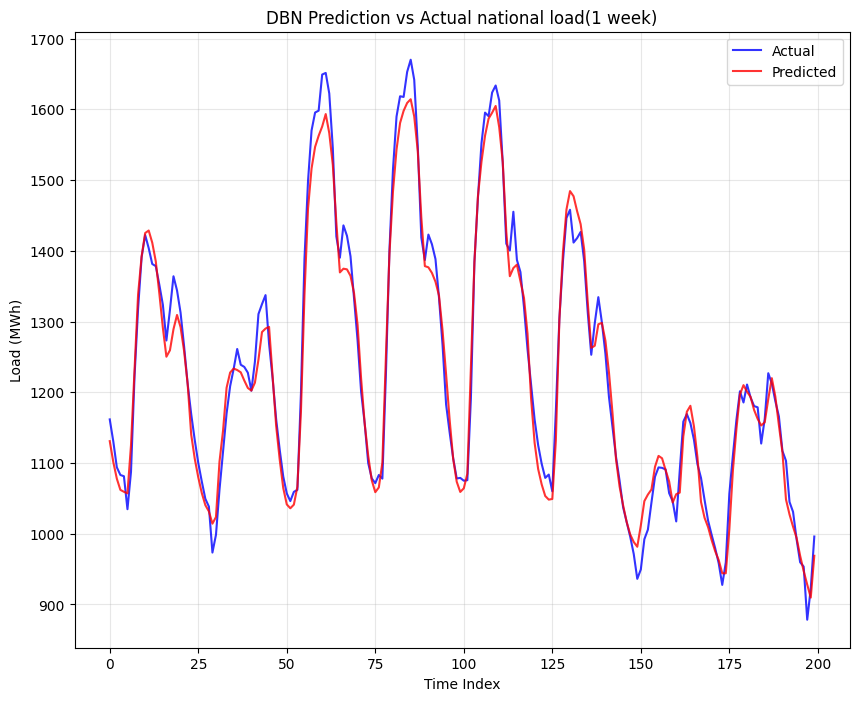
\includegraphics[width=\linewidth]{Chapters/images/results/DBN_predicted_vs_actual}
  		\caption{Predicted vs Actual load over a 1 week period of DBN}
  		\label{fig:dbnpredictedvsactual}
  	\end{minipage}
  	\hfill
  	\begin{minipage}[b]{0.45\linewidth}
  		\centering
  		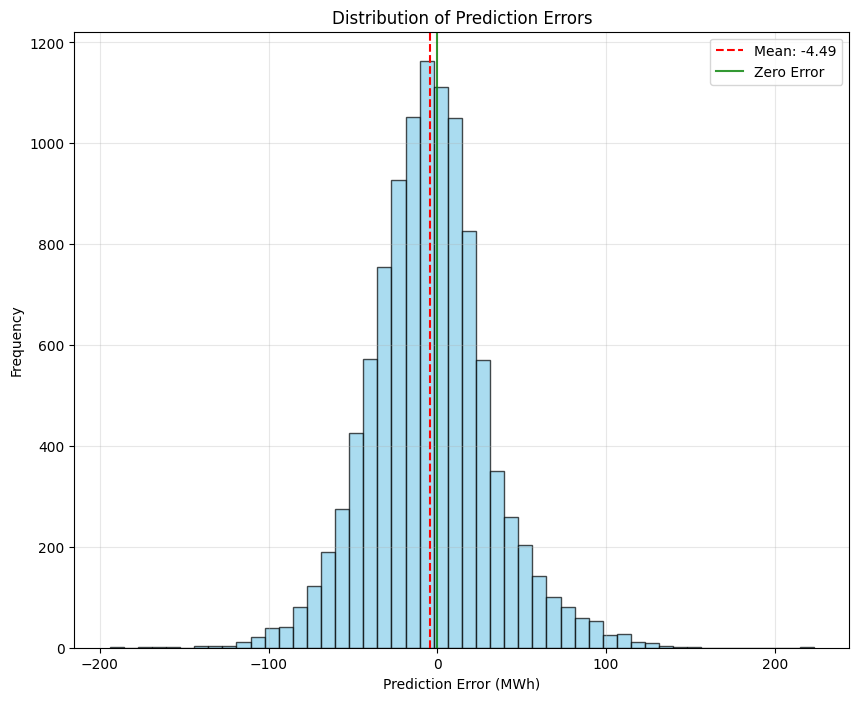
\includegraphics[width=\linewidth]{Chapters/images/results/dbn_error_distribution}
  		\caption{Distribution of prediction errors for the DBN model}
  		\label{fig:dbnerrordistribution}
  	\end{minipage}
  	
  \end{figure}
  
Figure \ref{fig:dbnpredictedvsactual} shows that the predicted load values closely follow the actual demand, with minimal deviation across the observed period. The error distribution in Figure \ref{fig:dbnerrordistribution} further supports this, displaying a near normal distribution centered around zero indicating that most prediction errors are small and unbiased.  
  \begin{figure}[h!]
  	\centering
  	\includegraphics[width=0.4\linewidth]{"Chapters/images/results/dbn_validation loss"}
  	\caption{DBN model loss during training and validation}
  	\label{fig:dbnvalidation-loss}
  \end{figure}
  Finally, the loss curves in Figure \ref{fig:dbnvalidation-loss} confirm stable convergence during training, with training decreasing steadily before flattening out and validation losses decreasing erratically but further flattening out. This behavior demonstrates effective learning and generalization without significant overfitting.
  
 
 
 \subsection{Deep Learning : CNN model results}
 
 The CNN model achieved a Test MAPE of 2.89\% and an $R^2$ value of 0.93, demonstrating strong predictive performance comparable to the DBN model. Table \ref{tab:cnn_performance_diff} summarizes the model’s training and testing performance metrics. The comparison between the two phases helps assess the model’s generalization capability and identify potential overfitting.
 \begin{table}[h!]
 	\small
 	\centering
 	\caption{Performance Metrics of the CNN Model}
 	\label{tab:cnn_performance_diff}
 	\begin{tabular}{lccc}
 		\hline
 		\textbf{Metric} & \textbf{Training} & \textbf{Test} & \textbf{Difference} \\
 		\hline
 		MAPE (\%) & 1.4700 & 2.887 & +1.4170 \\
 		MAE (Mwh) & 16.713 & 33.976& +16.364 \\
 		RMSE (Mwh) & 25.282 & 33.976 & +8.6946 \\
 		R$^2$ & 0.9827 & 0.9250 & -0.0578 \\
 		MSE & 639.17 & 2564.2 & +1925.0 \\
 		\hline
 	\end{tabular}
 \end{table}
The results show a moderate increase in error metrics between the training and testing sets, suggesting that the model generalized reasonably well without significant overfitting. Although the $R^2$ values are high, this does not necessarily indicate overfitting. As discussed by Plevris et al. \cite{plevris2022investigation}, the $R^2$ metric can increase with the addition of more input features, even if some of these features have limited correlation with the target variable. In this study, the inclusion of engineered temporal and statistical features likely contributed to the elevated $R^2$ value observed.
\begin{figure}[h!]
	\centering
	\begin{minipage}[b]{0.46\linewidth}
	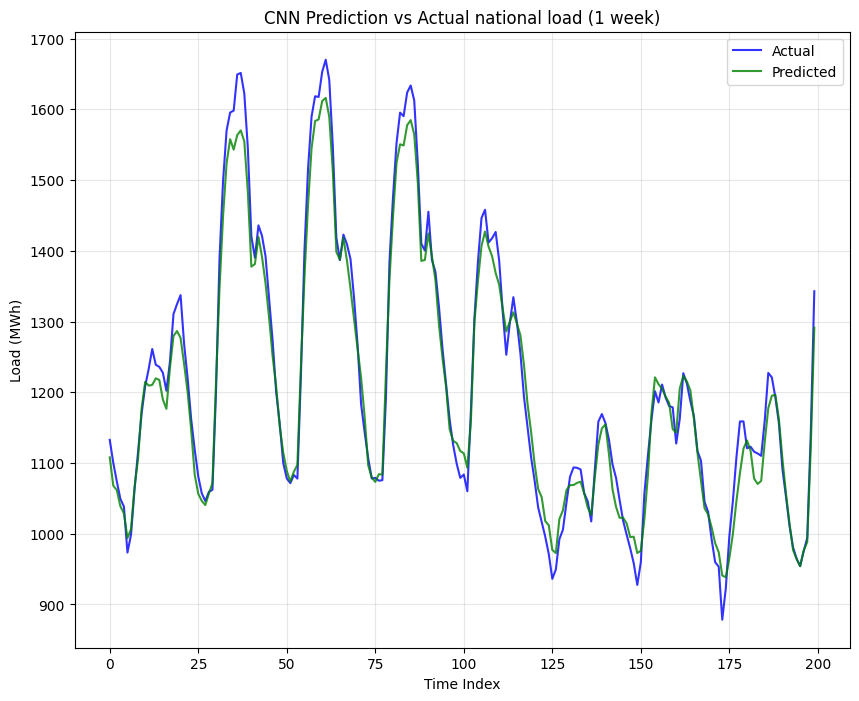
\includegraphics[width=\linewidth]{Chapters/images/results/cnn_predictionvsactual}
	\caption{The predicted and actual loading from the CNN model}
	\label{fig:cnnpredictionvsactual}
	\end{minipage}
	\begin{minipage}[b]{0.46\linewidth}
	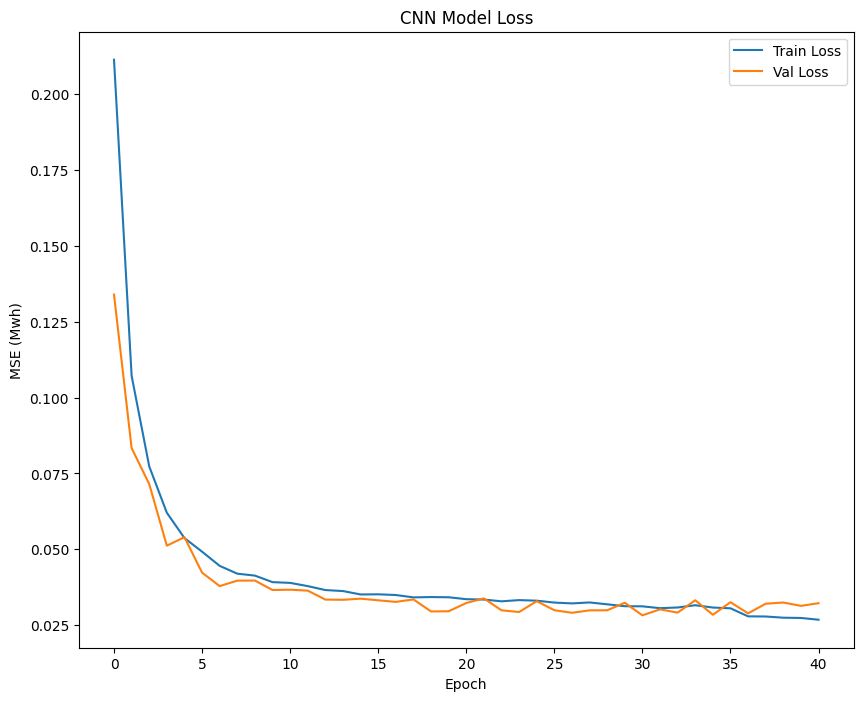
\includegraphics[width=\linewidth]{Chapters/images/results/CNN_model_loss}
	\caption{The CNN model validation and test loss against the epochs}
	\label{fig:cnnmodelloss}
	\end{minipage}
\end{figure}
Figure \ref{fig:cnnmodelloss} illustrates the training and validation loss curves across epochs. The training loss decreases steadily, indicating effective learning of spatial patterns within the input data. However, the validation loss exhibits slight fluctuations and does not converge smoothly, suggesting that the model may be somewhat sensitive to variations in the validation data. This behaviour could be attributed to the limited dataset size or the complex, non-linear nature of the short-term load data.

As shown in Figure \ref{fig:cnnpredictionvsactual}, the predicted load closely follows the actual demand, confirming the CNN model’s ability to capture key short-term variations and underlying load profiles. Overall, the CNN demonstrated strong predictive capability and generalization, effectively learning spatial dependencies from the structured time-series data while maintaining competitive accuracy relative to the other models tested.

\subsection{LSTM model results}
The LSTM model outperformed ES model, achieving a MAPE of 2.82\% and a MAE of 33.48 MWh. These results indicate that the model was able to effectively capture the temporal dependencies and nonlinear characteristics of the load data. The full set of performance metrics is presented in Table \ref{tab:lstm_performance}.
\begin{table}[h!]
	\centering
	
	\begin{tabular}{lc}
		\hline
		\textbf{Metric} & \textbf{Value} \\
		\hline
		MSE (Mwh) & 2319 \\
		RMSE(Mwh)&48.016 \\
	MAE (Mwh)& 33.48 \\
	$R^2$ (\%)& 0.933 \\
	MAPE & 2.82\% \\
		\hline
	\end{tabular}
	\caption{LSTM Model Performance Metrics}
	\label{tab:lstm_performance}
\end{table}
The low MSE and RMSE values reflect a well-fitting model with minimal deviation between predicted and actual load values. The high $R^2$ score of 0.933 demonstrates strong generalization capability and suggests that the LSTM effectively captured underlying temporal trends in the data.
\begin{figure}[h!]
	\centering
	\includegraphics[width=0.9\linewidth]{"Chapters/images/results/lstm_model loss"}
	\caption{The LSTM model loss during training and validation}
	\label{fig:lstmmodel-loss}
\end{figure}
Figure \ref{fig:lstmmodel-loss} shows the training and validation loss curves, indicating stable convergence and the absence of overfitting. Both losses decrease smoothly and plateau without significant fluctuations, confirming that the model successfully learned the data patterns without memorizing noise.
\begin{figure}[h!]
	\centering
	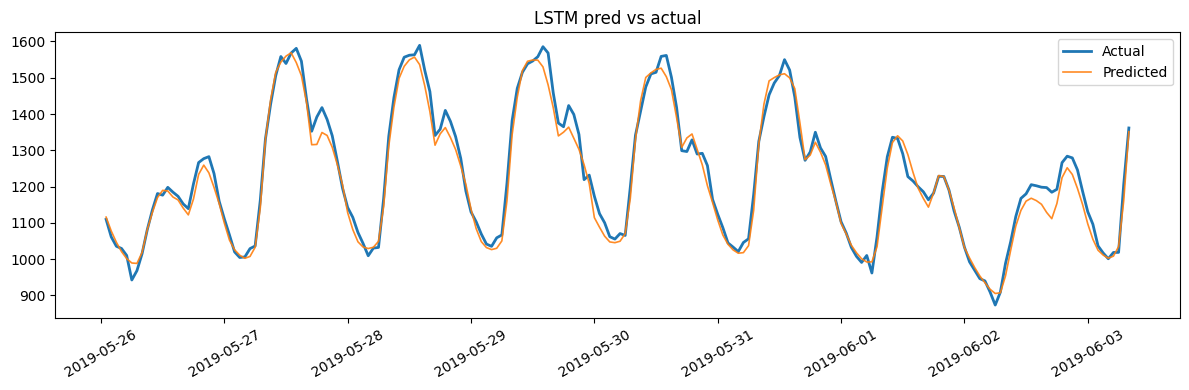
\includegraphics[width=0.5\linewidth]{Chapters/images/results/lstm_predicted_vs_actual}
	\caption{Comparison of the predicted LSTM output vs the actual demand}
	\label{fig:lstmpredictedvsactual}
\end{figure}
As shown in Figure \ref{fig:lstmpredictedvsactual}, the predicted values closely follow the actual load demand over a one-week period, demonstrating the model’s ability to track short-term fluctuations in energy consumption accurately. This result highlights the LSTM’s strength in modeling nonlinear, sequential dependencies, making it well-suited for short-term load forecasting tasks.

\subsection{Hybrid Model : CNN-LSTM Model Results}
The hybrid CNN-LSTM model achieved a MAPE of 2.90\% and a MAE of 34.63 MWh on the test dataset. The detailed performance metrics are presented in Table \ref{tab:cnn-lstm-results}.
  \begin{table}[h!]
 	\centering
 	\caption{Performance Metrics of the CNN Model}
 	\label{tab:cnn-lstm-results}
 	\begin{tabular}{lccc}
 		\hline
 		\textbf{Metric} & \textbf{Test} \\
 		\hline
 		MAPE (\%) &  2.902 \\
 		MAE (Mwh) &   34.63  \\
 		RMSE (Mwh) &  48.60  \\
 		R$^2$ &  0.929  \\
 		MSE & 2464  \\
 		\hline
 	\end{tabular}
 \end{table}
 \begin{figure}[h!]
 	\centering
 	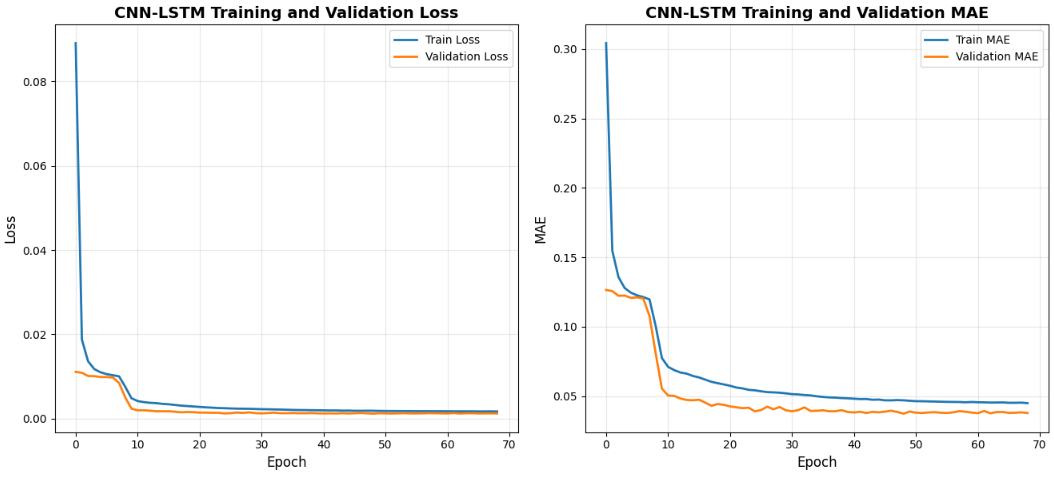
\includegraphics[width=0.9\linewidth,height=0.3\textwidth]{Chapters/images/results/CNN-LSTM-MODEL-LOSS}
 	\caption{Model train and validation loss over 69 epochs.}
 	\label{fig:cnn-lstm-model-loss}
 \end{figure}
Figure \ref{fig:cnn-lstm-model-loss} shows a settling in the training and validation loss. The MAE loss it also below the train MAE which shows normalcy in the training process. 
 \begin{figure}[h!]
 	\centering
 	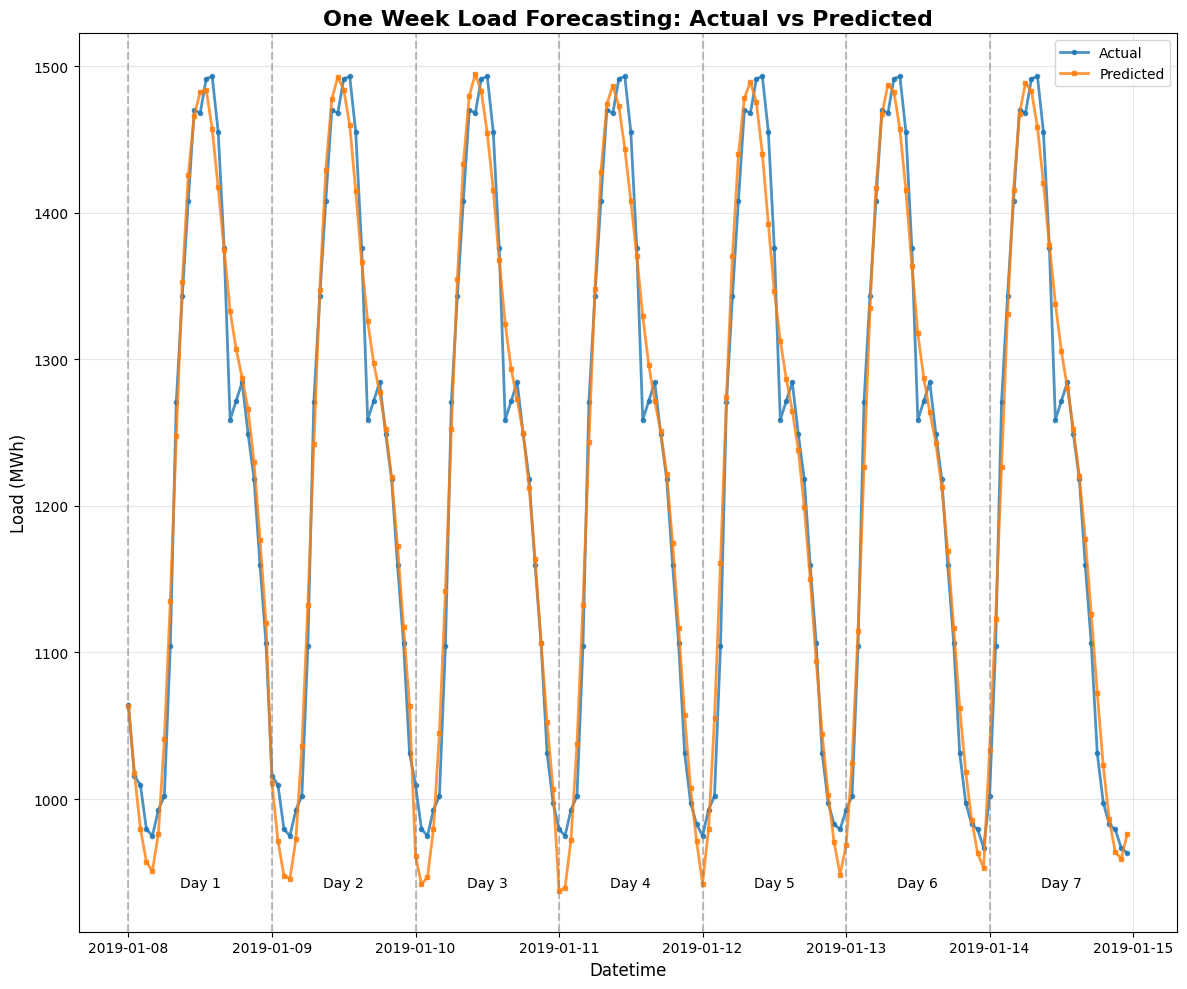
\includegraphics[width=0.9\linewidth,height=0.38\textwidth]{Chapters/images/results/cnn_lstm_prediction_vs_actual}
 	\caption{comparison of predicted vs actual load in a CNN-LSTM model}
 	\label{fig:cnnlstmpredictionvsactual}
 \end{figure}
 
Figure \ref{fig:cnnlstmpredictionvsactual} presents a one-week comparison between the predicted and actual load demand. The predicted curve closely follows the actual load trend, indicating that the hybrid model captures temporal dependencies effectively within short-term horizons. However, when evaluated over the entire dataset (Figure \ref{fig:cnnlstmpredictionvsactualfull}), it becomes evident that the model underperforms in specific periods—particularly during sudden drops or fluctuations in demand.
 \begin{figure}[h]
 	\centering
 	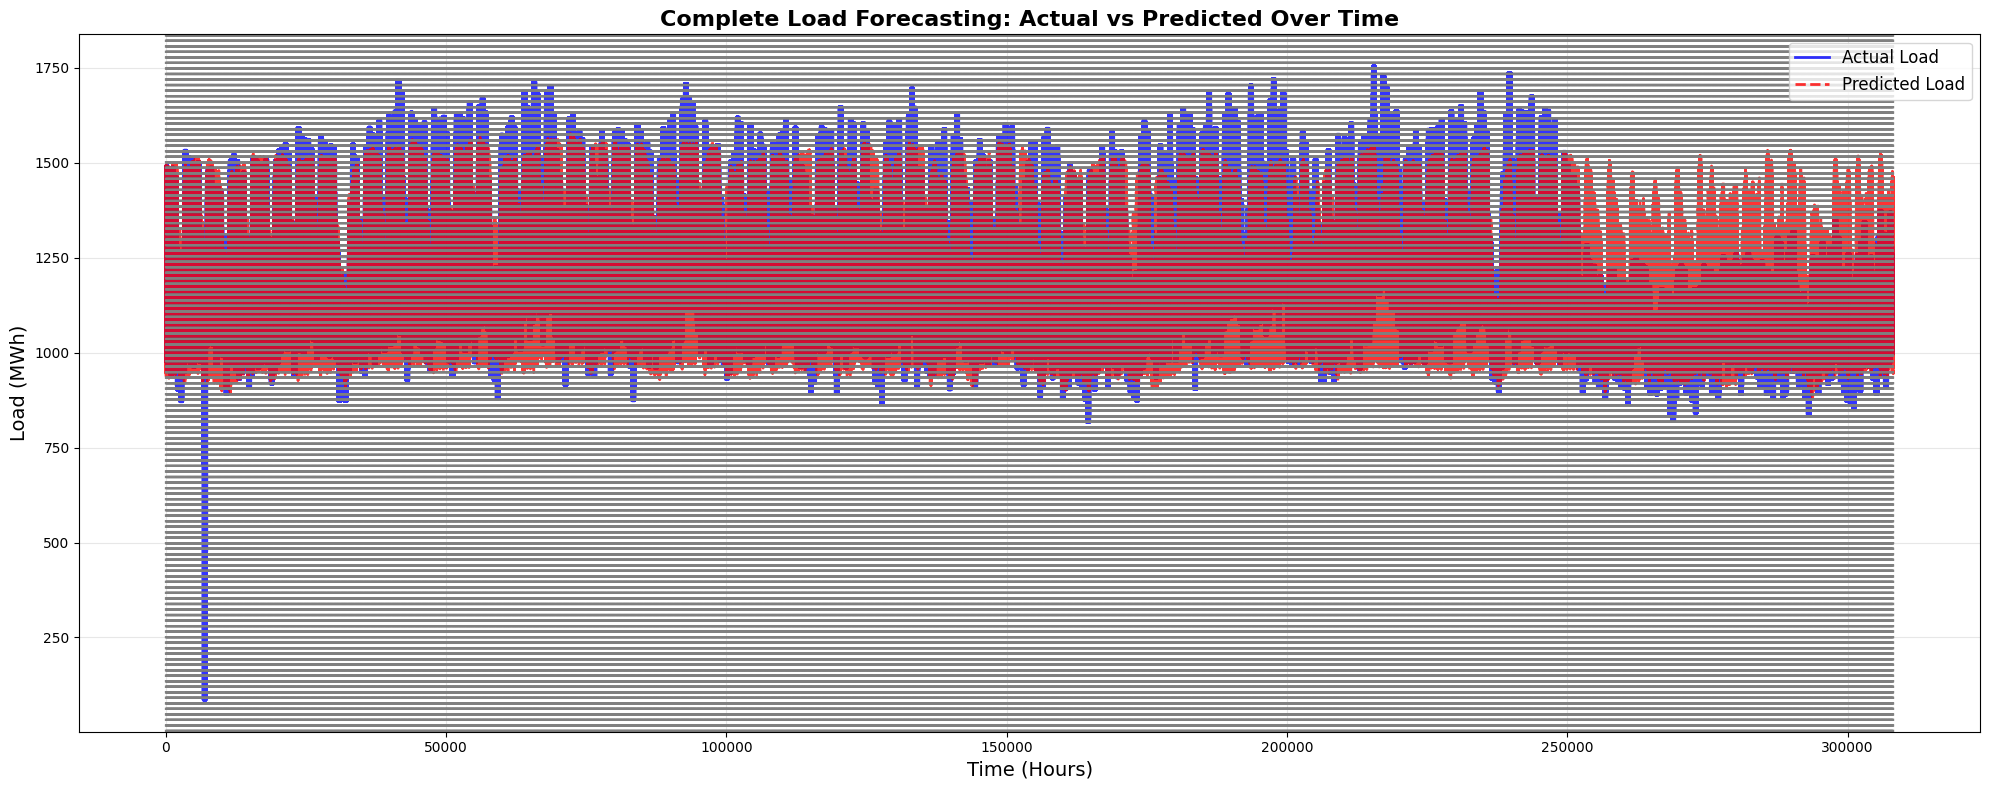
\includegraphics[width=0.9\linewidth,height=0.3\textwidth]{Chapters/images/results/cnn_lstm_prediction_vs_actual_full}
 	\caption{The complete comparison of the CNN-LSTMs predicted vs actual demand}
 	\label{fig:cnnlstmpredictionvsactualfull}
 \end{figure}
 
 
 \section{Comparative Results}
 
The six models tested in this research were trained and tested on data with an 80/20 train-test split. The validation was set to a 20\% of the testing data. The performance metrics of the models have been captured in Table \ref{tab:model-performance}. The table contains the MAPE values which show the XGBoost model performing the best amongst all the models. The ES model however had the highest MAPE representing a lack of generalization of the model, this is also further backed by its $r^2$ value.
\begin{table}[htbp]
 	\centering
 	\small
 	\caption{Performance comparison of forecasting models}
 	\label{tab:model-performance}
 	
 	\resizebox{\textwidth}{!}{%
 	\begin{tabular}{lrrrrr}
 		\hline
 		\textbf{Model} & \textbf{MSE (Mwh)} & \textbf{MAE (MwH)} & \textbf{MAPE (\%)} & \textbf{RMSE (Mwh)} & \textbf{R\textsuperscript{2}} \\
 		\hline
 		Exponential Smoothing & 20,118 & 118.14 & 9.57 & 141.84 & 0.5241 \\
 		XGBoost               & 719.58 & 19.06  & 1.598 & 26.82  & 0.979  \\
 		DBN                   & 1,160  & 24.87  & 2.1   & 34.06  & 0.966  \\
 		CNN                   & 2,564  & 33.97  & 2.887 & 50.64  & 0.925  \\
 		LSTM                  & 2,319  & 33.48  & 2.82  & 48.016 & 0.933  \\
 		CNN-LSTM              & 2,464  & 34.63  & 2.902 & 48.64  & 0.929  \\
 		\hline
 	\end{tabular}}
 \end{table}
 From Table \ref{tab:model-performance}, the XGBoost model achieved the best overall performance with the lowest MAPE 1.598\% and MAE 19.06 MWh, while the ES model performed the worst, showing weak generalization and the lowest $R^2$ value 0.5241. Among the deep learning models, the DBN outperformed both the CNN and LSTM, achieving a MAPE of 2.1\% compared to 2.89\% and 2.82\% respectively. The hybrid CNN-LSTM model yielded only a marginal improvement, achieving a MAPE of 2.9\%, which was slightly higher than its component models.
 
 To visualize these results, Figures \ref{fig:rmsecomparison}, \ref{fig:maecomparison}, and \ref{fig:mapecomparison1} present a comparison of RMSE, MAE, and MAPE values across all models. These visualizations reinforce the numerical results, highlighting the superior performance of XGBoost and the comparatively weak performance of the ES model.
 
 \begin{figure}[h]
 	\centering
 	\begin{minipage}[b]{0.325\linewidth}
 		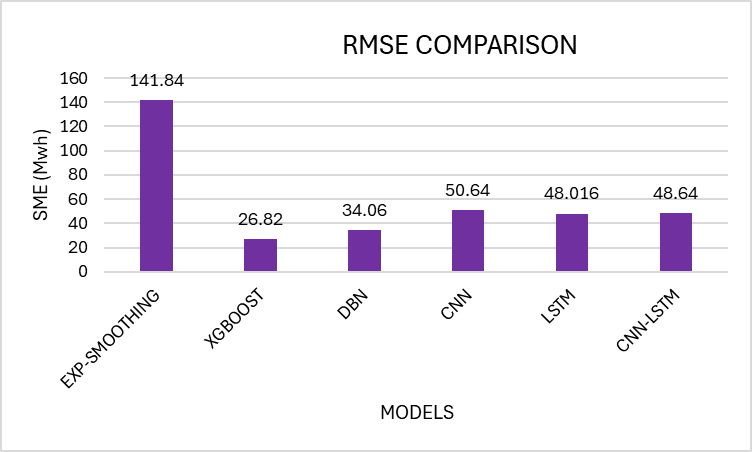
\includegraphics[width=\linewidth]{Chapters/images/results/RMSE_COMPARISON}
 		\caption{RMSE Comparison}
 		\label{fig:rmsecomparison}
 	\end{minipage}
 	\begin{minipage}[b]{0.325\linewidth}
 		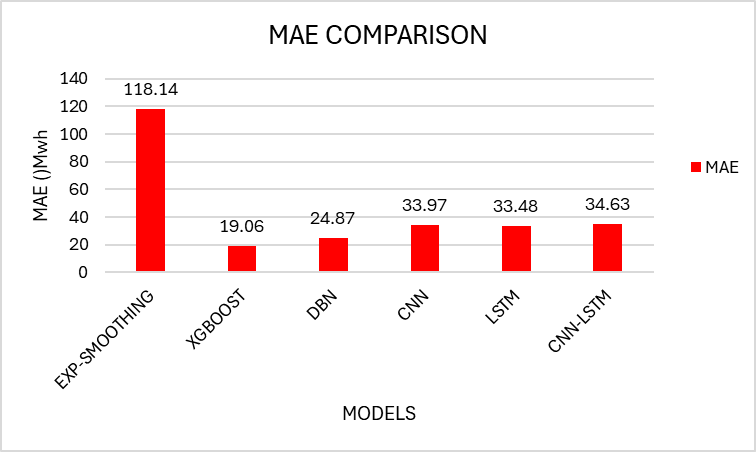
\includegraphics[width=\linewidth]{Chapters/images/results/MAE_COMPARISON}
 		\caption{MAE Comparison}
 		\label{fig:maecomparison}
 	\end{minipage}
 	\begin{minipage}[b]{0.325\linewidth}
 		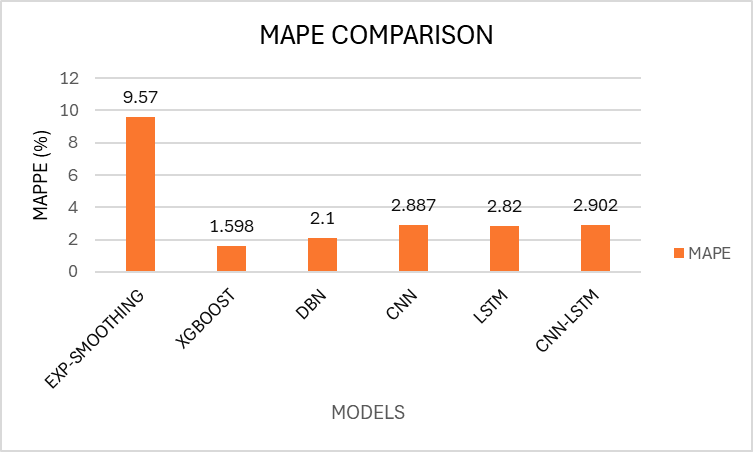
\includegraphics[width=\linewidth]{Chapters/images/results/MAPE_COMPARISON1}
 		\caption{MAPE Comparison}
 		\label{fig:mapecomparison1}
 	\end{minipage}
 \end{figure}
 
Figure \ref{fig:xgboostvsexpsmoothing} compares the XGBoost and ES model forecasts against the actual load over three days. The XGBoost model closely follows the actual demand profile, while the ES model lags during peak load periods, explaining its higher MAPE and RMSE values.

 \begin{figure}[h!]
 	\centering
 	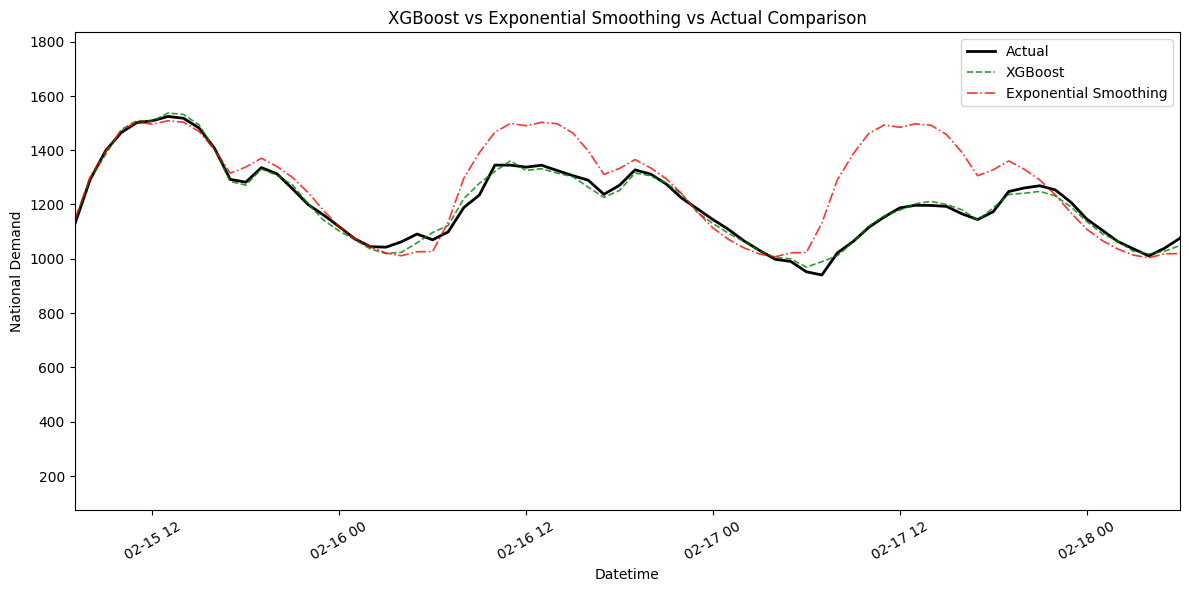
\includegraphics[width=0.75\linewidth]{Chapters/images/results/xgboost_vs_expsmoothing}
 	\caption{XGBoost vs ES and the actual load}
 	\label{fig:xgboostvsexpsmoothing}
 \end{figure}
 
 The performance of the DBN and CNN models, both of which utilize deep feature extraction, is compared in Figure \ref{fig:cnnvsdbnactual}. While both models track the actual load well, the DBN demonstrates smoother adaptation during dips, consistent with its lower MAPE and higher $R^2$. 
 \begin{figure}[h!]
 	\centering
 	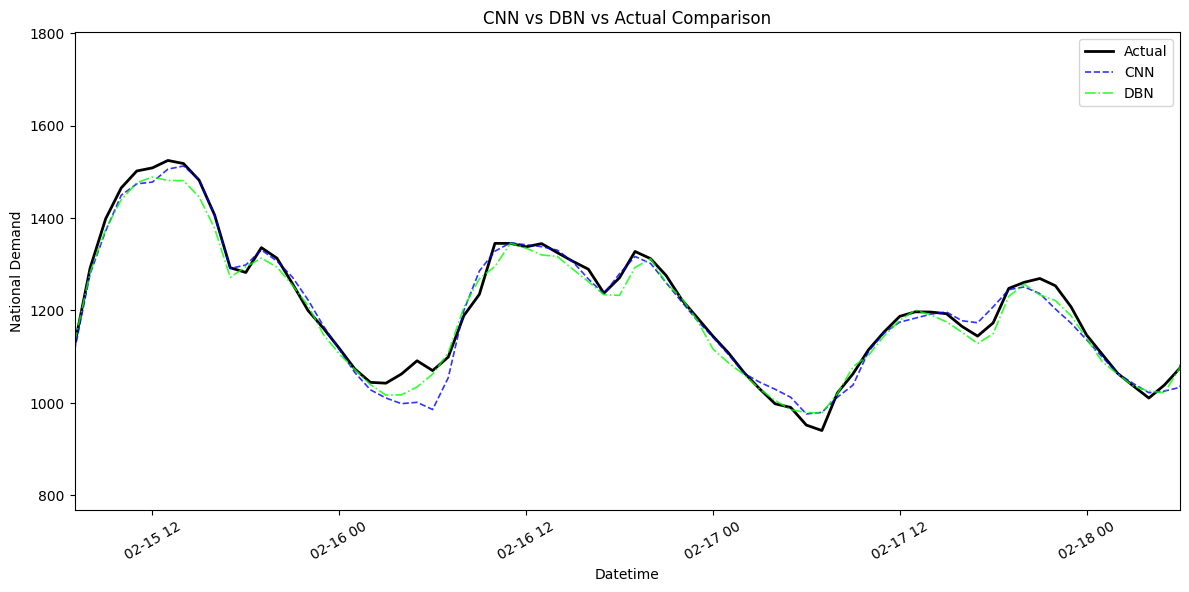
\includegraphics[width=0.75\linewidth]{Chapters/images/results/cnn_vs_dbn_actual}
 	\caption{DBN compared to CNN}
 	\label{fig:cnnvsdbnactual}
 \end{figure}
 
 The DBN and CNN have a similar neural network architecture with multilevel features on both models. Their performance was also compared to each other and in figure \ref{fig:cnnvsdbnactual} the models are compared to each other. Table \ref{tab:model-performance} shows the DBN outperforming the CNN on all performance parameters and this is also highlighted in figure \ref{fig:cnnvsdbnactual}. The two models trace the actual load very well however the CNN model fails to trace at certain points on dips. The difference is negligible though as the difference in their MAPE values is 0.7\%.
 \begin{figure}[h!]
 	\centering
 	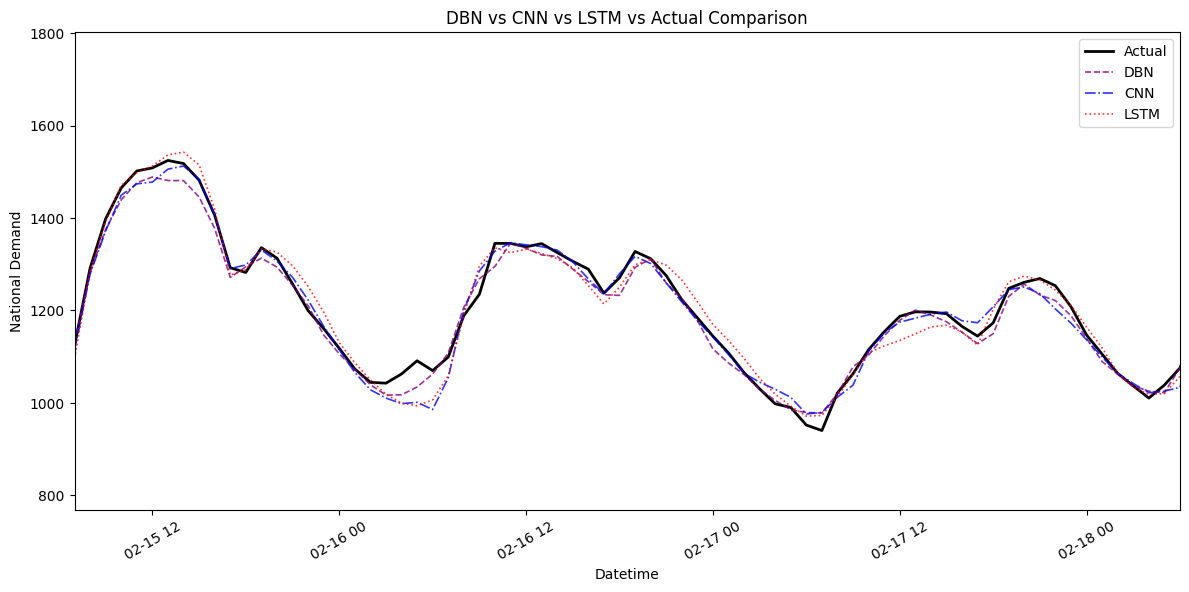
\includegraphics[width=0.75\linewidth]{Chapters/images/results/cnn_vs_dbn_vs_lstm_vs_actual}
 	\caption{DBN, CNN, LSTM and actual compared to each other}
 	\label{fig:cnnvsdbnvslstmvsactual}
 \end{figure}
 
 Further comparison among the deep learning models DBN, CNN, and LSTM is shown in Figure \ref{fig:cnnvsdbnvslstmvsactual}. All models capture general demand trends effectively, though the CNN and LSTM tend to underperform during sudden drops in load.
 
 Further in the comparison of the models in figure \ref{fig:cnnvsdbnvslstmvsactual} compares the Deep learning models usd in the research. The performance metrics shows that the DBN performs best with a MAPE of 2.1\% while LSTM and CNN trail close behind with 2.82\% and 2.89\% respectively. Figure \ref{fig:cnnvsdbnvslstmvsactual} shows the three models tracing the actual load. IT however shows the CNN and LSTM trailing behind on the dips which is expected because of their higher MAPE, MAE and RMSE values.
  \begin{figure}[h!]
 	\centering
 	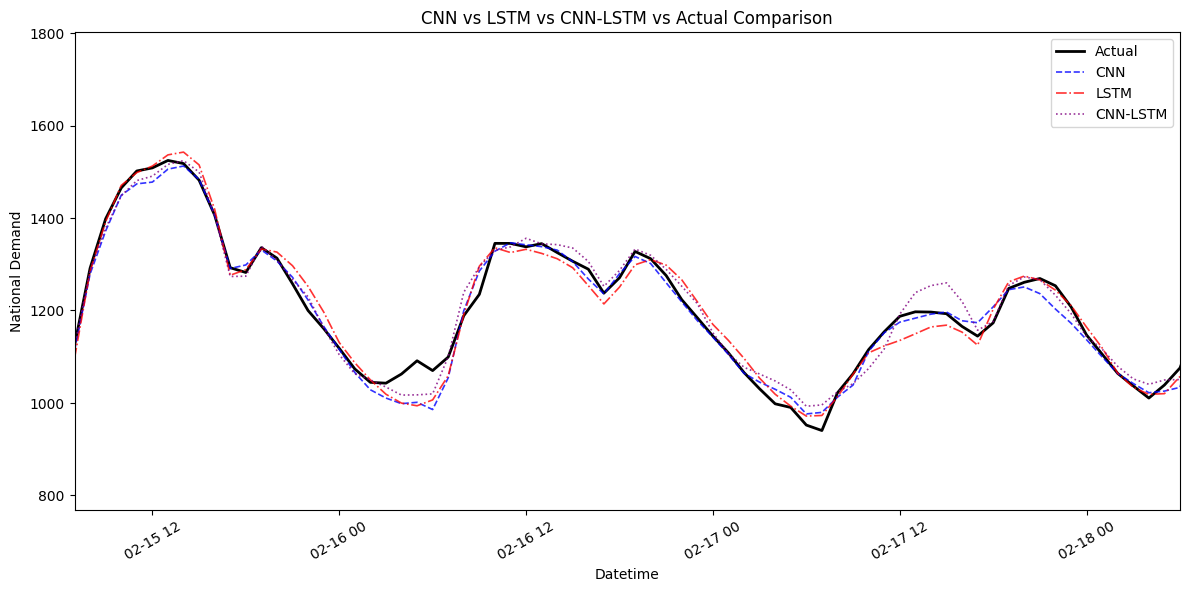
\includegraphics[width=0.75\linewidth]{Chapters/images/results/cnn_vs_lstm_vs_cnn-lstm_vs_actual}
 	\caption{CNN, LSTM, CNN-LSTM compared to each other}
 	\label{fig:cnnvslstmvscnn-lstmvsactual}
 \end{figure}
 

The hybrid CNN-LSTM model was expected to outperform the standalone CNN and LSTM due to its combined spatial and temporal learning capabilities. However, as shown in Figure \ref{fig:cnnvslstmvscnn-lstmvsactual}, the hybrid model achieved only a marginal improvement. While it demonstrated localized accuracy improvements in certain regions, its overall performance metrics indicate no substantial gain.
\begin{figure}[h]
 	\centering
 	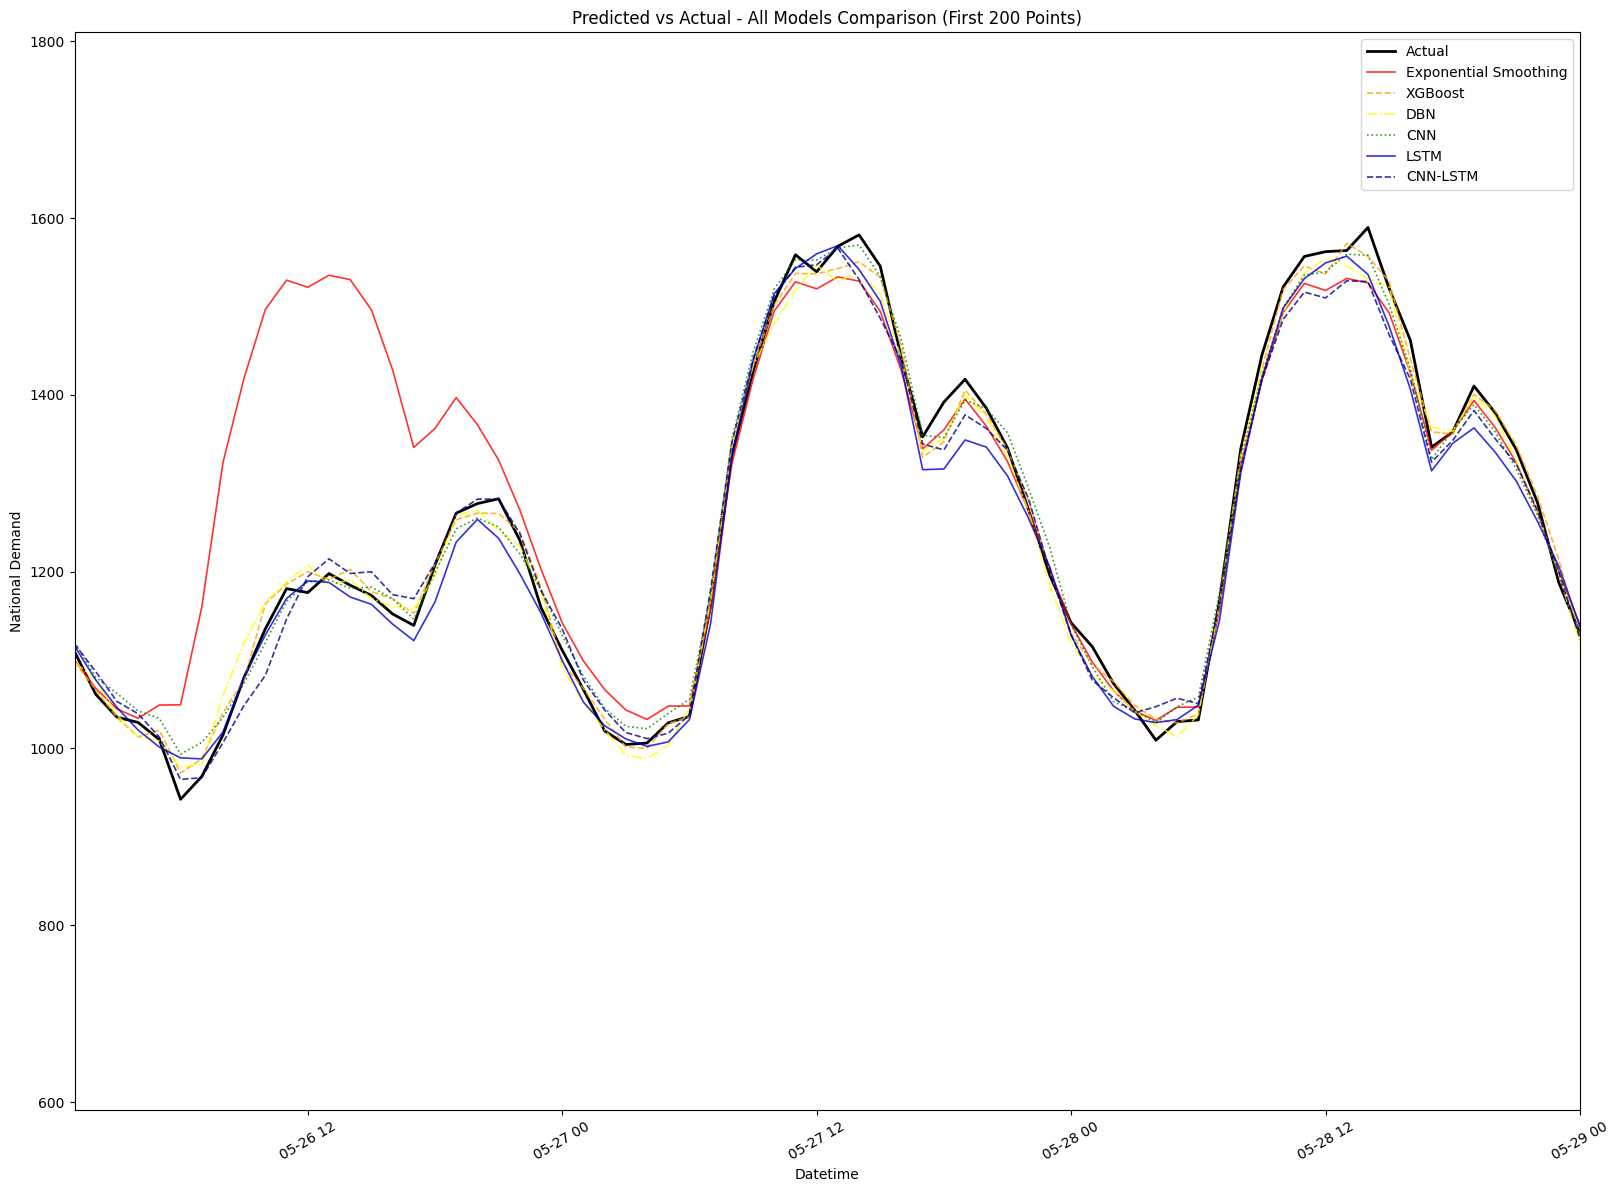
\includegraphics[width=0.8\linewidth]{Chapters/images/results/all_model_comparison}
 	\caption{performance comparison of 6 models}
 	\label{fig:allmodelcomparison}
 \end{figure}

  
  
 Finally, Figure \ref{fig:allmodelcomparison} summarizes the performance of all six models over the full evaluation period. The XGBoost and DBN models consistently trace the actual load with minimal deviation, while the ES model shows high sensitivity to variations in demand. The CNN-based models demonstrate strong pattern recognition but struggle to generalize on peaks and troughs. These results collectively support the effectiveness of machine learning and deep learning techniques in short-term load forecasting, with tree-based ensemble methods like XGBoost showing the most reliable performance.
  
  
 